%----------------------------------------------------------------------------------------
%	Capítulo 6
%----------------------------------------------------------------------------------------

\pagestyle{myportland}
\doublespacing
%\pagenumbering{arabic}
\chapter[\quad\quad\quad\quad ----- Pruebas y resultados]{\\ Pruebas y resultados}
\thispagestyle{myportland}

Este capítulo está enfocado en mostrar simulaciones o pruebas obtenidas en los algoritmos o mecanismos empleados en el sistema. Además desarrolla de manera técnica los resultados con la finalidad de ser comparables con resultados de otros autores de otras máquinas.

%% NUEVA SECCIÓN X.X
\section{Algoritmos de clasificación y conteo de truchas}

El algoritmo presentado basado en la arquitectura de redes neuronales convolucionales denominada YOLO permite hacer inferencias sobre las imágenes. Con la versión 3 de esta arquitectura que sigue bajo desarrollo actualmente para mejorar el rendimiento. Las inferencias permiten detectar objetos para los cuales la red es entrenada mediante una gran cantidad de imágenes que contienen el objeto de interés. Para el procesamiento básicamente se realiza un redimensionamiento de la imagen antes de procesarla, luego diferentes arquitecturas de redes neuronales dentro de la arquitectura logran detectar el objeto. Luego de detectado el objeto se procede a segmentarlo mediante técnicas de enmascarado de objetos. Finalmente cada objeto detectado en la imagen es contabilizado dentro del programa. En la Figura \ref{fig:pruebas algoritmo} se muestra en el lado izquierdo la imagen que se ingresa al algoritmo y a la derecha el pez segmentado para ser contabilizado.

\begin{myfigure}[H]
	\footnotesize\centering
	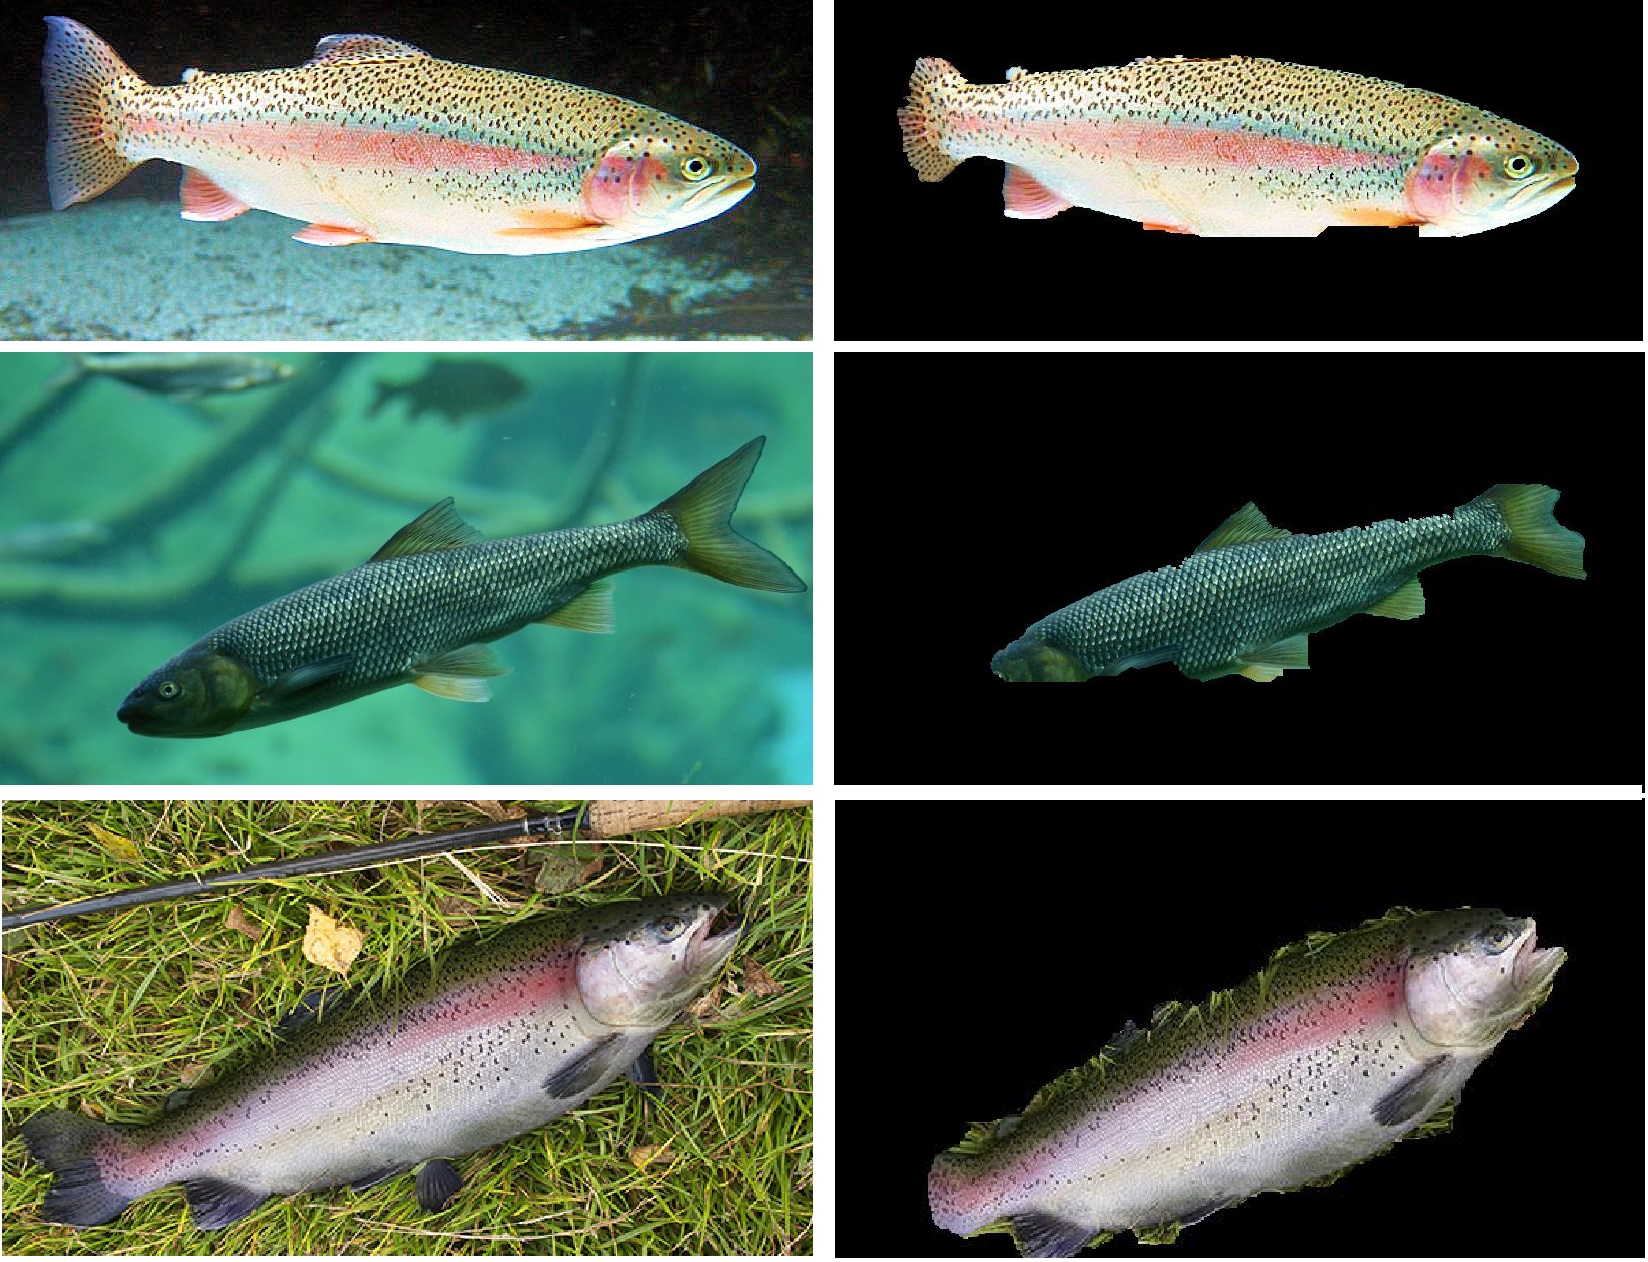
\includegraphics[width=1\textwidth]{chapter6/pruebas algoritmo.png}
	\caption{Inferencia de detección y conteo de truchas.}
	\begin{myflushcenter}
		Fuente: Elaboración propia.
	\end{myflushcenter}
	\label{fig:pruebas algoritmo}
\end{myfigure}

En el caso de la clasificación el sistema debe ser calibrado acorde al entorno, por lo que su etapa de desarrollo luego de la detección se da en la etapa de prototipado y producción. Sin embargo, el conteo es realizado sin ningún problema.

%% NUEVA SECCIÓN X.X.X
\subsection{Definición de criterios de clasificación}

\textcolor{blue}{[BORRADOR] Lorem ipsum dolor sit amet, consectetur adipiscing elit, sed do eiusmod tempor incididunt ut labore et dolore magna aliqua. Lacus sed turpis tincidunt id aliquet. Nunc aliquet bibendum enim facilisis gravida neque convallis a. Ut tellus elementum sagittis vitae et leo duis ut diam. Dolor sit amet consectetur adipiscing elit ut aliquam purus sit. Dolor sed viverra ipsum nunc aliquet bibendum. Euismod in pellentesque massa placerat. Et malesuada fames ac turpis egestas sed tempus urna. Euismod elementum nisi quis eleifend quam adipiscing vitae proin. Ornare suspendisse sed nisi lacus sed. Mollis aliquam ut porttitor leo a diam. Varius morbi enim nunc faucibus. Sit amet purus gravida quis blandit turpis cursus in hac. [/BORRADOR]} 

%% NUEVA SECCIÓN X.X.X
\subsection{Análisis de tiempo de ejecución del algoritmo}

\textcolor{blue}{[BORRADOR] Lorem ipsum dolor sit amet, consectetur adipiscing elit, sed do eiusmod tempor incididunt ut labore et dolore magna aliqua. Lacus sed turpis tincidunt id aliquet. Nunc aliquet bibendum enim facilisis gravida neque convallis a. Ut tellus elementum sagittis vitae et leo duis ut diam. Dolor sit amet consectetur adipiscing elit ut aliquam purus sit. Dolor sed viverra ipsum nunc aliquet bibendum. Euismod in pellentesque massa placerat. Et malesuada fames ac turpis egestas sed tempus urna. Euismod elementum nisi quis eleifend quam adipiscing vitae proin. Ornare suspendisse sed nisi lacus sed. Mollis aliquam ut porttitor leo a diam. Varius morbi enim nunc faucibus. Sit amet purus gravida quis blandit turpis cursus in hac. [/BORRADOR]} 

%% NUEVA SECCIÓN X.X.X
%\subsection{Errores detectados en la simulación de conteo de truchas}

%\textcolor{blue}{[BORRADOR] Lorem ipsum dolor sit amet, consectetur adipiscing elit, sed do eiusmod tempor incididunt ut labore et dolore magna aliqua. Lacus sed turpis tincidunt id aliquet. Nunc aliquet bibendum enim facilisis gravida neque convallis a. Ut tellus elementum sagittis vitae et leo duis ut diam. Dolor sit amet consectetur adipiscing elit ut aliquam purus sit. Dolor sed viverra ipsum nunc aliquet bibendum. Euismod in pellentesque massa placerat. Et malesuada fames ac turpis egestas sed tempus urna. Euismod elementum nisi quis eleifend quam adipiscing vitae proin. Ornare suspendisse sed nisi lacus sed. Mollis aliquam ut porttitor leo a diam. Varius morbi enim nunc faucibus. Sit amet purus gravida quis blandit turpis cursus in hac. [/BORRADOR]} 

%% NUEVA SECCIÓN X.X
\section{Simulación estructural}
		
%\textcolor{blue}{[BORRADOR] Explicar selección entre otras cosas .... Además, citar a \cite{ChinchayDeLaCruz2010} en análisis de falla de levas [/BORRADOR]}

\textcolor{blue}{[BORRADOR] Lorem ipsum dolor sit amet, consectetur adipiscing elit, sed do eiusmod tempor incididunt ut labore et dolore magna aliqua. Lacus sed turpis tincidunt id aliquet. Nunc aliquet bibendum enim facilisis gravida neque convallis a. Ut tellus elementum sagittis vitae et leo duis ut diam. Dolor sit amet consectetur adipiscing elit ut aliquam purus sit. Dolor sed viverra ipsum nunc aliquet bibendum. Euismod in pellentesque massa placerat. Et malesuada fames ac turpis egestas sed tempus urna. Euismod elementum nisi quis eleifend quam adipiscing vitae proin. Ornare suspendisse sed nisi lacus sed. Mollis aliquam ut porttitor leo a diam. Varius morbi enim nunc faucibus. Sit amet purus gravida quis blandit turpis cursus in hac. [/BORRADOR]} 


%% NUEVA SECCIÓN X.X
\section{Simulación dinámica del sistema}

\textcolor{blue}{[BORRADOR] Lorem ipsum dolor sit amet, consectetur adipiscing elit, sed do eiusmod tempor incididunt ut labore et dolore magna aliqua. Lacus sed turpis tincidunt id aliquet. Nunc aliquet bibendum enim facilisis gravida neque convallis a. Ut tellus elementum sagittis vitae et leo duis ut diam. Dolor sit amet consectetur adipiscing elit ut aliquam purus sit. Dolor sed viverra ipsum nunc aliquet bibendum. Euismod in pellentesque massa placerat. Et malesuada fames ac turpis egestas sed tempus urna. Euismod elementum nisi quis eleifend quam adipiscing vitae proin. Ornare suspendisse sed nisi lacus sed. Mollis aliquam ut porttitor leo a diam. Varius morbi enim nunc faucibus. Sit amet purus gravida quis blandit turpis cursus in hac. [/BORRADOR]} 


